\chapter{Entrepreneurship Development Program}
\ifpdf
    \graphicspath{{Chapter3/Chapter3Figs/PNG/}{Chapter3/Chapter3Figs/PDF/}{Chapter3/Chapter3Figs/}}
\else
    \graphicspath{{Chapter3/Chapter3Figs/EPS/}{Chapter3/Chapter3Figs/}}
\fi

\section{About}
Entrepreneurship Development Program was started at Synergy Sansthan with the help of ``Pravah'', a NGO based in Delhi. As the name suggests, it is related to developing entrepreneurial skills in individuals. 

\subsection{Goals}
The goals of EDP are to equip small and medium scale entrepreneurs with the skills needed to make their business bloom. To help them in procuring loans from the bank rather than from money lenders who would extort them. To make them independent eventually by making their business profitable for them.


\begin{figure}[ht!]
  \begin{center}
    \leavevmode
    \ifpdf
      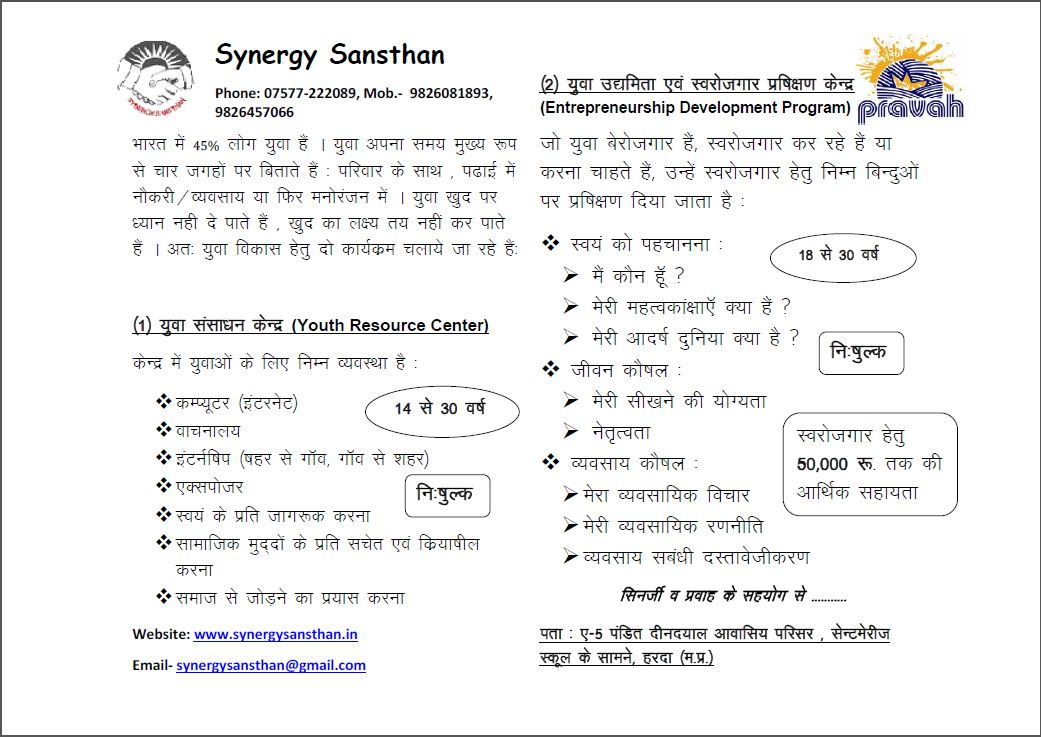
\includegraphics[width=6.5in]{pamphlet}
    \else
      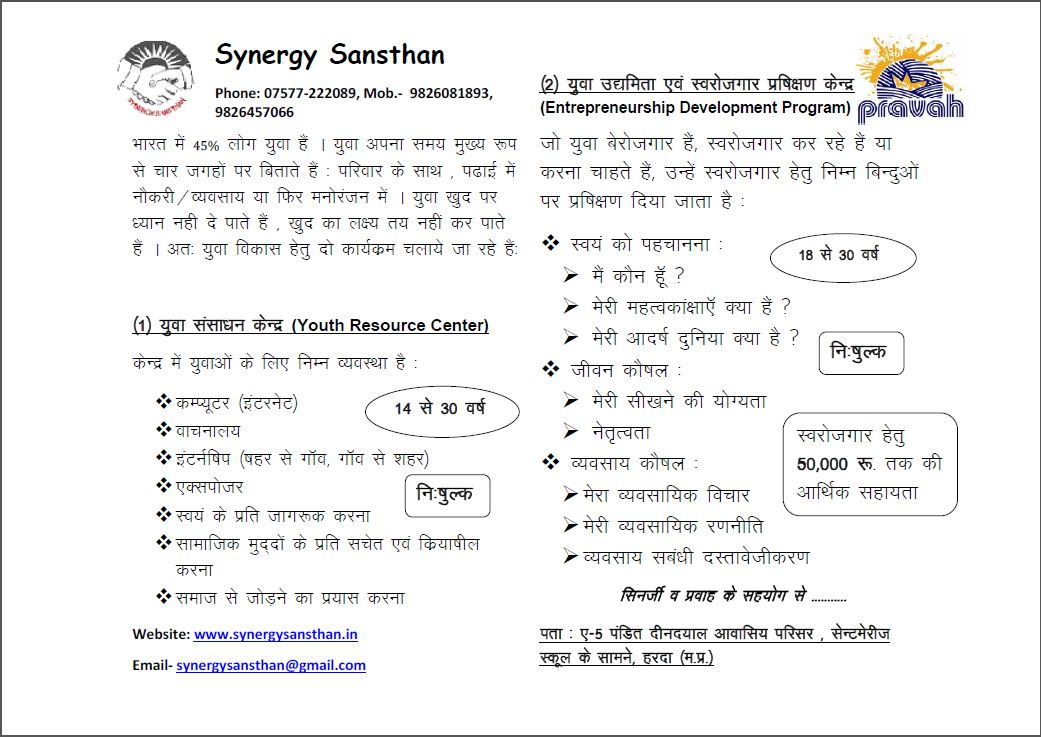
\includegraphics[bb = 92 86 545 742, height=6in]{pamphlet}
    \fi
    \caption{EDP Pamphlet}
    \label{FigAir}
  \end{center}
\end{figure}

\subsection{Methods}
The applicants would be given training on different aspects of business management. They would be told about how to maximize their profits and ubderstand their shortcomings. Apart from the analysis, Synergy Sansthan would Help in making all the proper paper work of the individuals. This would allow them to get loans from the bank at proper interest rates. A sustainable model would also be set up for them so that they can grow better.
% \subsubsection{first subsub section in the second subsection}
% ... and some more in the first subsub section otherwise it all looks the same
% doesn't it? well we can add some text to it ...

% \subsection{third subsection in the First Section}
% ... and some more ...

% \subsubsection{first subsub section in the third subsection}
% ... and some more in the first subsub section otherwise it all looks the same
% doesn't it? well we can add some text to it and some more and some more and
% some more and some more and some more and some more and some more ...

% \subsubsection{second subsub section in the third subsection}
% ... and some more in the first subsub section otherwise it all looks the same
% doesn't it? well we can add some text to it ...

\section{Mobilizing Strategies}
% \markboth{\MakeUppercase{\thechapter. My Third Chapter }}{\thechapter. My Third Chapter}
The mobilization strategy consisted of 5 steps as follows:
\begin{enumerate}
	\item \textbf{Mind Jog} \newline
		Ask them the goal of their life.
	\item \textbf{Personal Connection} \newline
		Ask the individual why did he start the business.
	\item \textbf{Information Exchange} \newline
		Tell them that India has 40-45\% youth and only 3\% of them get jobs. 
	\item \textbf{Information Application} \newline
		Tell them about the EDP.
	\item \textbf{Real World Connection} \newline
		Tell them the benefits of EDP and everything it has to offer.
\end{enumerate}




\section{Case Study}

\subsection{Rajiv Jat - Photocopy shop}
Rajiv Jat ran a small photocopy shop in Harda city. His daily business was of Rs. 150. He faced a lot of difficulty in supporting his family. Synergy Sansthan helped him out in setting his business properly. They got him a loan so that he could purchase 1 computer for his shop and get Internet access. This allowed him to have a small cyber-cafe. This enhanced his business considerably as the number of people having Internet access in Harda were very few.


\begin{figure}[ht!]
  \begin{center}
    \leavevmode
    \ifpdf
      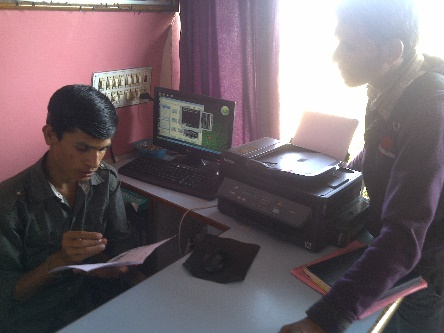
\includegraphics[width=4in]{computerguy}
    \else
      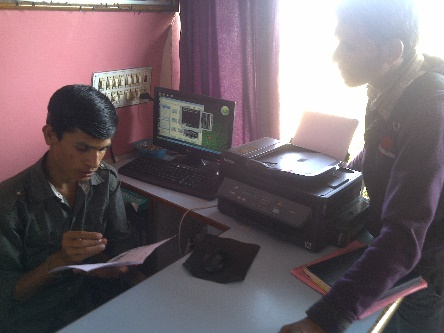
\includegraphics[bb = 92 86 545 742, height=6in]{computerguy}
    \fi
    \caption{Rajiv Jat - Photocopy shop}
    \label{FigAir}
  \end{center}
\end{figure}

% ------------------------------------------------------------------------


%%% Local Variables: 
%%% mode: latex
%%% TeX-master: "../thesis"
%%% End: 
